\subsection{Cracking Minesweeper with Z3 SMT solver}
\label{minesweeper_SMT}

For those who are not very good at playing Minesweeper (like me), it's possible to predict bombs' placement without touching debugger.

Here is a clicked somewhere and I see revealed empty cells and cells with known number of "neighbours":

\begin{figure}[H]
\centering
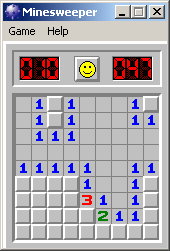
\includegraphics[scale=0.75]{SMT/minesweeper/1.png}
\end{figure}

What we have here, actually? Hidden cells, empty cells (where bombs are not present), and empty cells with numbers, which shows how many bombs are placed nearby.
Here is what we can do: we will try to place a bomb to all possible hidden cells and ask Z3 SMT solver, if it can disprove the very fact that the bomb can be placed there.

\subsubsection{The method}

Take a look at this fragment. "?" mark is for unknown cell, "." is for empty cell, digit is a number of neighbours.

\begin{lstlisting}
_PRE_BEGIN
? ? ?
? 3 .
? 1 .
\end{lstlisting}

So there are 5 unknown cells.
We will try each unknown cell by placing a bomb there.
Let's first pick top/left cell:

\begin{lstlisting}
1 ? ?
? 3 .
? 1 .
\end{lstlisting}

Then we will try to solve the following system of equations (\textit{RrCc} is cell of row r and column c):

\begin{lstlisting}
R1C2+R2C1+R2C2=1                               (because we placed bomb at R1C1)	
R2C1+R2C2+R3C1=1                               (because we have "1" at R3C2)	
R1C1+R1C2+R1C3+R2C1+R2C2+R2C3+R3C1+R3C2+R3C3=3 (because we have "3" at R2C2)	
R1C2+R1C3+R2C2+R2C3+R3C2+R3C3=0                (because we have "." at R2C3)	
R2C2+R2C3+R3C2+R3C3=0                          (because we have "." at R3C3)
\end{lstlisting}

As it turns out, this system of equations is satisfiable, so there could be a bomb at this cell.
But this information is not interesting to us, since we want to find cells we can freely click on.
And we will try another one...

\subsubsection{The code}

\lstinputlisting{SMT/minesweeper/minesweeper_solver.py}

The code is almost self-explanatory.
We need border for the same reason, why Conway's "Game of Life" implementations also has border (to make calculation
function simpler).
Whenever we know that the cell is free of bomb, we put zero there.
Whenever we know number of neighbours, we add a constraint, again, just like in "Game of Life": number of neighbours must be equal to the number we got from the Minesweeper.
Then we place bomb somewhere and check.

Let's run:

\begin{lstlisting}
row=1 col=3, unsat!
row=6 col=2, unsat!
row=6 col=3, unsat!
row=7 col=4, unsat!
row=7 col=9, unsat!
row=8 col=9, unsat!
\end{lstlisting}

These are cells where I can click safely, so I did:

\begin{figure}[H]
\centering
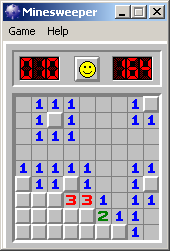
\includegraphics[scale=0.75]{SMT/minesweeper/2.png}
\end{figure}

Now we have more information, so we update input:

\begin{lstlisting}
known=[
"01110001?",
"01?100011",
"011100000",
"000000000",
"111110011",
"?11?1001?",
"???331011",
"?????2110",
"???????10"]
\end{lstlisting}

I run it again:

\begin{lstlisting}
row=7 col=1, unsat!
row=7 col=2, unsat!
row=7 col=3, unsat!
row=8 col=3, unsat!
row=9 col=5, unsat!
row=9 col=6, unsat!
\end{lstlisting}

I click on these cells again:

\begin{figure}[H]
\centering
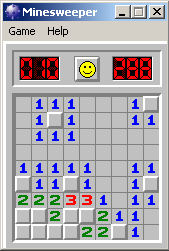
\includegraphics[scale=0.75]{SMT/minesweeper/3.png}
\end{figure}

I update it again:

\begin{lstlisting}
known=[
"01110001?",
"01?100011",
"011100000",
"000000000",
"111110011",
"?11?1001?",
"222331011",
"??2??2110",
"????22?10"]
\end{lstlisting}

\begin{lstlisting}
row=8 col=2, unsat!
row=9 col=4, unsat!
\end{lstlisting}

\begin{figure}[H]
\centering
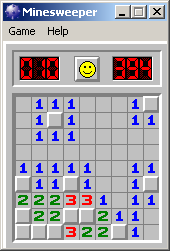
\includegraphics[scale=0.75]{SMT/minesweeper/4.png}
\end{figure}

This is last update:

\begin{lstlisting}
known=[
"01110001?",
"01?100011",
"011100000",
"000000000",
"111110011",
"?11?1001?",
"222331011",
"?22??2110",
"???322?10"]
\end{lstlisting}

... last result:

\begin{lstlisting}
row=9 col=1, unsat!
row=9 col=2, unsat!
\end{lstlisting}

Voila!

\begin{figure}[H]
\centering
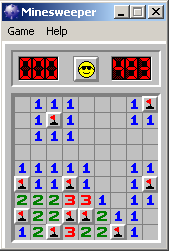
\includegraphics[scale=0.75]{SMT/minesweeper/5.png}
\end{figure}

The source code: \url{https://github.com/dennis714/SAT_SMT_article/blob/master/SMT/minesweeper/minesweeper_solver.py}.

Some discussion on HN: \url{https://news.ycombinator.com/item?id=13797375}.

See also: cracking it using SAT solver: \ref{minesweeper_SAT}.

